\documentclass{article}
\usepackage[utf8x]{inputenc}
\usepackage{ucs}
\usepackage{amsmath} 
\usepackage{amsfonts}
\usepackage{marvosym}
\usepackage{wasysym}
\usepackage{upgreek}
\usepackage[english,russian]{babel}
\usepackage{graphicx}
\usepackage{float}
\usepackage{textcomp}
\usepackage{hyperref}
\usepackage{geometry}
  \geometry{left=2cm}
  \geometry{right=1.5cm}
  \geometry{top=1cm}
  \geometry{bottom=2cm}
\usepackage{tikz}
\usepackage{ccaption}
\usepackage{multicol}

\hypersetup{
   colorlinks=true,
   citecolor=blue,
   linkcolor=black,
   urlcolor=blue
}

\usepackage{listings}
%\setlength{\columnsep}{1.5cm}
%\setlength{\columnseprule}{0.2pt}

\usepackage[absolute]{textpos}

\usepackage{colortbl,graphicx,tikz}
\definecolor{X}{rgb}{.5,.5,.5}

\renewcommand{\thesubsection}{\arabic{subsection}}

\begin{document}
\pagenumbering{gobble}
\lstset{
  language=C,                % choose the language of the code
  basicstyle=\linespread{1.1}\ttfamily,
  columns=fixed,
  fontadjust=true,
  basewidth=0.5em,
  keywordstyle=\color{blue}\bfseries,
  commentstyle=\color{gray},
  stringstyle=\ttfamily\color{orange!50!black},
  showstringspaces=false,
  numbersep=5pt,
  numberstyle=\tiny\color{black},
  numberfirstline=true,
  stepnumber=1,                   % the step between two line-numbers.        
  numbersep=10pt,                  % how far the line-numbers are from the code
  backgroundcolor=\color{white},  % choose the background color. You must add \usepackage{color}
  showstringspaces=false,         % underline spaces within strings
  captionpos=b,                   % sets the caption-position to bottom
  breaklines=true,                % sets automatic line breaking
  breakatwhitespace=true,         % sets if automatic breaks should only happen at whitespace
  xleftmargin=.2in,
  extendedchars=\true,
  keepspaces = true,
}
\lstset{literate=%
   *{0}{{{\color{red!20!violet}0}}}1
    {1}{{{\color{red!20!violet}1}}}1
    {2}{{{\color{red!20!violet}2}}}1
    {3}{{{\color{red!20!violet}3}}}1
    {4}{{{\color{red!20!violet}4}}}1
    {5}{{{\color{red!20!violet}5}}}1
    {6}{{{\color{red!20!violet}6}}}1
    {7}{{{\color{red!20!violet}7}}}1
    {8}{{{\color{red!20!violet}8}}}1
    {9}{{{\color{red!20!violet}9}}}1
}


\section*{Задачи на строки:}
\begin{center}
\scalebox{1}{ 
\begin{tabular}{cc | cc | cc | cc | cc | cc | cc | cc | cc | cc} 
\rowcolor[rgb]{0,0.173,0.3255}
\textcolor{white}{Symbol}&\textcolor{white}{Code}&
\textcolor{white}{S}&\textcolor{white}{C}&
\textcolor{white}{S}&\textcolor{white}{C}&
\textcolor{white}{S}&\textcolor{white}{C}&
\textcolor{white}{S}&\textcolor{white}{C}&
\textcolor{white}{S}&\textcolor{white}{C}&
\textcolor{white}{S}&\textcolor{white}{C}&
\textcolor{white}{S}&\textcolor{white}{C}&
\textcolor{white}{S}&\textcolor{white}{C}&
\textcolor{white}{S}&\textcolor{white}{C}
\\ 
\rowcolor[rgb]{0.89451,0.93588,0.97078} 
$\backslash$0 & 0  & \& & 38 & 0  & 48 & : & 58 & D & 68 & N & 78 & X & 88                & b & 98 & l & 108 & v & 118 \\
$\backslash$t & 9  & ' & 39 & 1   & 49 & ; & 59 & E & 69 & O & 79 & Y & 89                & c & 99 & m & 109 & w & 119 \\
\rowcolor[rgb]{0.89451,0.93588,0.97078} 
$\backslash$n & 10 & ( & 40 & 2   & 50 & < & 60 & F & 70 & P & 80 & Z & 90                & d & 100 & n & 110 & x & 120 \\
              &    & ) & 41 & 3   & 51 & = & 61 & G & 71 & Q & 81 & [ & 91                & e & 101 & o & 111 & y & 121 \\
              \rowcolor[rgb]{0.89451,0.93588,0.97078} 
(space)       & 32 & * & 42 & 4   & 52 & > & 62 & H & 72 & R & 82 & $\backslash$ & 92     & f & 102 & p & 112 & z & 122 \\
!             & 33 & + & 43 & 5   & 53 & ? & 63 & I & 73 & S & 83 & ] & 93                & g & 103 & q & 113 & \{ & 123 \\
\rowcolor[rgb]{0.89451,0.93588,0.97078} 
"             & 34 & , & 44 & 6   & 54 & @ & 64 & J & 74 & T & 84 & \textasciicircum & 94 & h & 104 & r & 114 & | & 124 \\
\#            & 35 & - & 45 & 7   & 55 & A & 65 & K & 75 & U & 85 & \_ & 95               & i & 105 & s & 115 & \} & 125 \\
\rowcolor[rgb]{0.89451,0.93588,0.97078} 
\$            & 36 & . & 46 & 8   & 56 & B & 66 & L & 76 & V & 86 & ` & 96                & j & 106 & t & 116 & \textasciitilde & 126 \\
\%            & 37 & / & 47 & 9   & 57 & C & 67 & M & 77 & W & 87 & a & 97                & k & 107 & u & 117 &  &  \\
 \end{tabular}
}
\end{center}

\subsection{Символы. Модификатор \%c:}
Символы - это числа типа \texttt{char}.\\
Функция \texttt{printf} с модификатором \%c принимает на вход число и печатает соответствующий символ.
\begin{lstlisting}
#include <stdio.h>
int main() {
	char x = 64;       // char - это число размером 1 байт ( от -128 до 127 )
	printf("%d\n", x); // печатаем число x
	printf("%c\n", x); // печатаем соответствующий символ
	
	// Символьные константы - символы в одинарных кавычках - это просто числа
	printf("%d\n", '>'); // Напечатает 62.  '>' == 65
	printf("%d\n", 'a' + '0'); // Напечатает 145
	printf("%d\n", '4'*'2');  // Что напечатает эта строка
}
\end{lstlisting}

\begin{itemize}
\item \textbf{ASCII:} Вывести на экран все символы таблицы ASCII с номерами от 32 до 126 в следующем формате: 
\begin{lstlisting}
Symbol = A, Code = 65
\end{lstlisting}
\item \textbf{Считывание символов:} Напишите программу, которая будет считывать символы один за другим в цикле \texttt{while} и печатать код каждого символа. Используйте scanf с модификатором \%c. Программа должна заканчиваться после ввода символа q.
\end{itemize}

\subsection{Строки. Модификатор \%s:}
Строки - это массивы чисел типа \texttt{char}. Обычные массивы нельзя печатать одной командой \texttt{printf}, но специально для строк ввели модификатор \texttt{\%s}, благодаря которому можно печатать и считывать строки одной командой.
\begin{lstlisting}
int main() {
	char a[20] = {77, 73, 80, 84, 0};
	char b[20] = {'M', 'I', 'P', 'T', '\0'};
	char c[20] = "MIPT"; // Лучше всего использовать эту инициализацию
	// Использовать = со строками можно только при создании, т.е. такое:
	a = "FAKI";  // работать не будет
	
	printf("%s\n", a);
	printf("%s\n", b);
	printf("%s\n", c);
}
\end{lstlisting}
\begin{itemize}
\item \textbf{Инициализация строки:} Объявите и инициализируйте строку \texttt{"Hello 11!"} 3-мя разными способами и напечатайте её.
\item \textbf{Изменение строки:} Измените созданную строку из прошлой задачи на \texttt{"Hello 12!"} и снова напечатайте её. Новую строку создавать не надо.
\item \textbf{Считывание строки:} Считайте число \texttt{n} и строку \texttt{str} и напечатайте её \texttt{n} раз через пробел.
\item \textbf{Удвоение:} Считайте строку и напечатайте её удвоив каждый символ. Для итерации используйте тот факт, что в конце строки всегда должен стоять нулевой символ (символ с кодом \texttt{0}).
\begin{center}
\begin{tabular}{ c | c }
 вход & выход \\ \hline
 Hello & HHeelllloo  \\ 
 MIPT & MMIIPPTT  \\ 
\end{tabular}
\end{center}
\item \textbf{Длина строки:} Напишите функцию \texttt{int get\_length(char* str)}, которая будет возвращать длину строки. Проверьте эту функцию в \texttt{main()}.
\item \textbf{Переворот:} Напишите функцию \texttt{void reverse\_string(char* str)}, которая будет переворачивать строку строку. Проверьте эту функцию в \texttt{main()}. Так как строка - это просто массив из чисел, то она передаётся в функцию по указателю (также как и обычный массив) и, соответственно может меняться внутри.
\begin{center}
\begin{tabular}{ c | c }
 вход & выход \\ \hline
 Hello! & !olleH  \\ 
 live & evil  \\ 
 Madam & madaM  \\ 
\end{tabular}
\end{center}

\item \textbf{UPPERCASE:} Напишите функцию \texttt{void to\_upper\_case(char* str)}, которая будет переводить строку в верхний регистр. Проверьте эту функцию в \texttt{main()}.
\begin{center}
\begin{tabular}{ c | c }
 вход & выход \\ \hline
 mipt & MIPT \\
 Hello! & HELLO!  \\ 
 Area51 & AREA51 \\
\end{tabular}
\end{center}

\item \textbf{Усечение строки:} На вход подаётся строка. Усечь строку до первого символа точка \texttt{``.''}. Можно использовать только один вызов функции printf().
\begin{center}
\begin{tabular}{ c | c }
 вход & выход \\ \hline
 judge.mipt.ru & judge \\
 A.B.C. & A  \\ 
\end{tabular}
\end{center}

Как вы могли заметить, использование scanf с модификатором \texttt{\%s} считывает одно слово. Чтобы считывать символы до переноса строки (то есть до символа '\textbackslash n'), следует использовать модификатор \verb|%[^\n]|.
\begin{lstlisting}
scanf("%[^\n]", str);
\end{lstlisting}

\item \textbf{Шифр Цезаря:} Шифр Цезаря — это вид шифра подстановки, в котором каждый символ заменяется символом, находящимся на некотором постоянном числе позиций левее или правее него в алфавите. 
\begin{center}
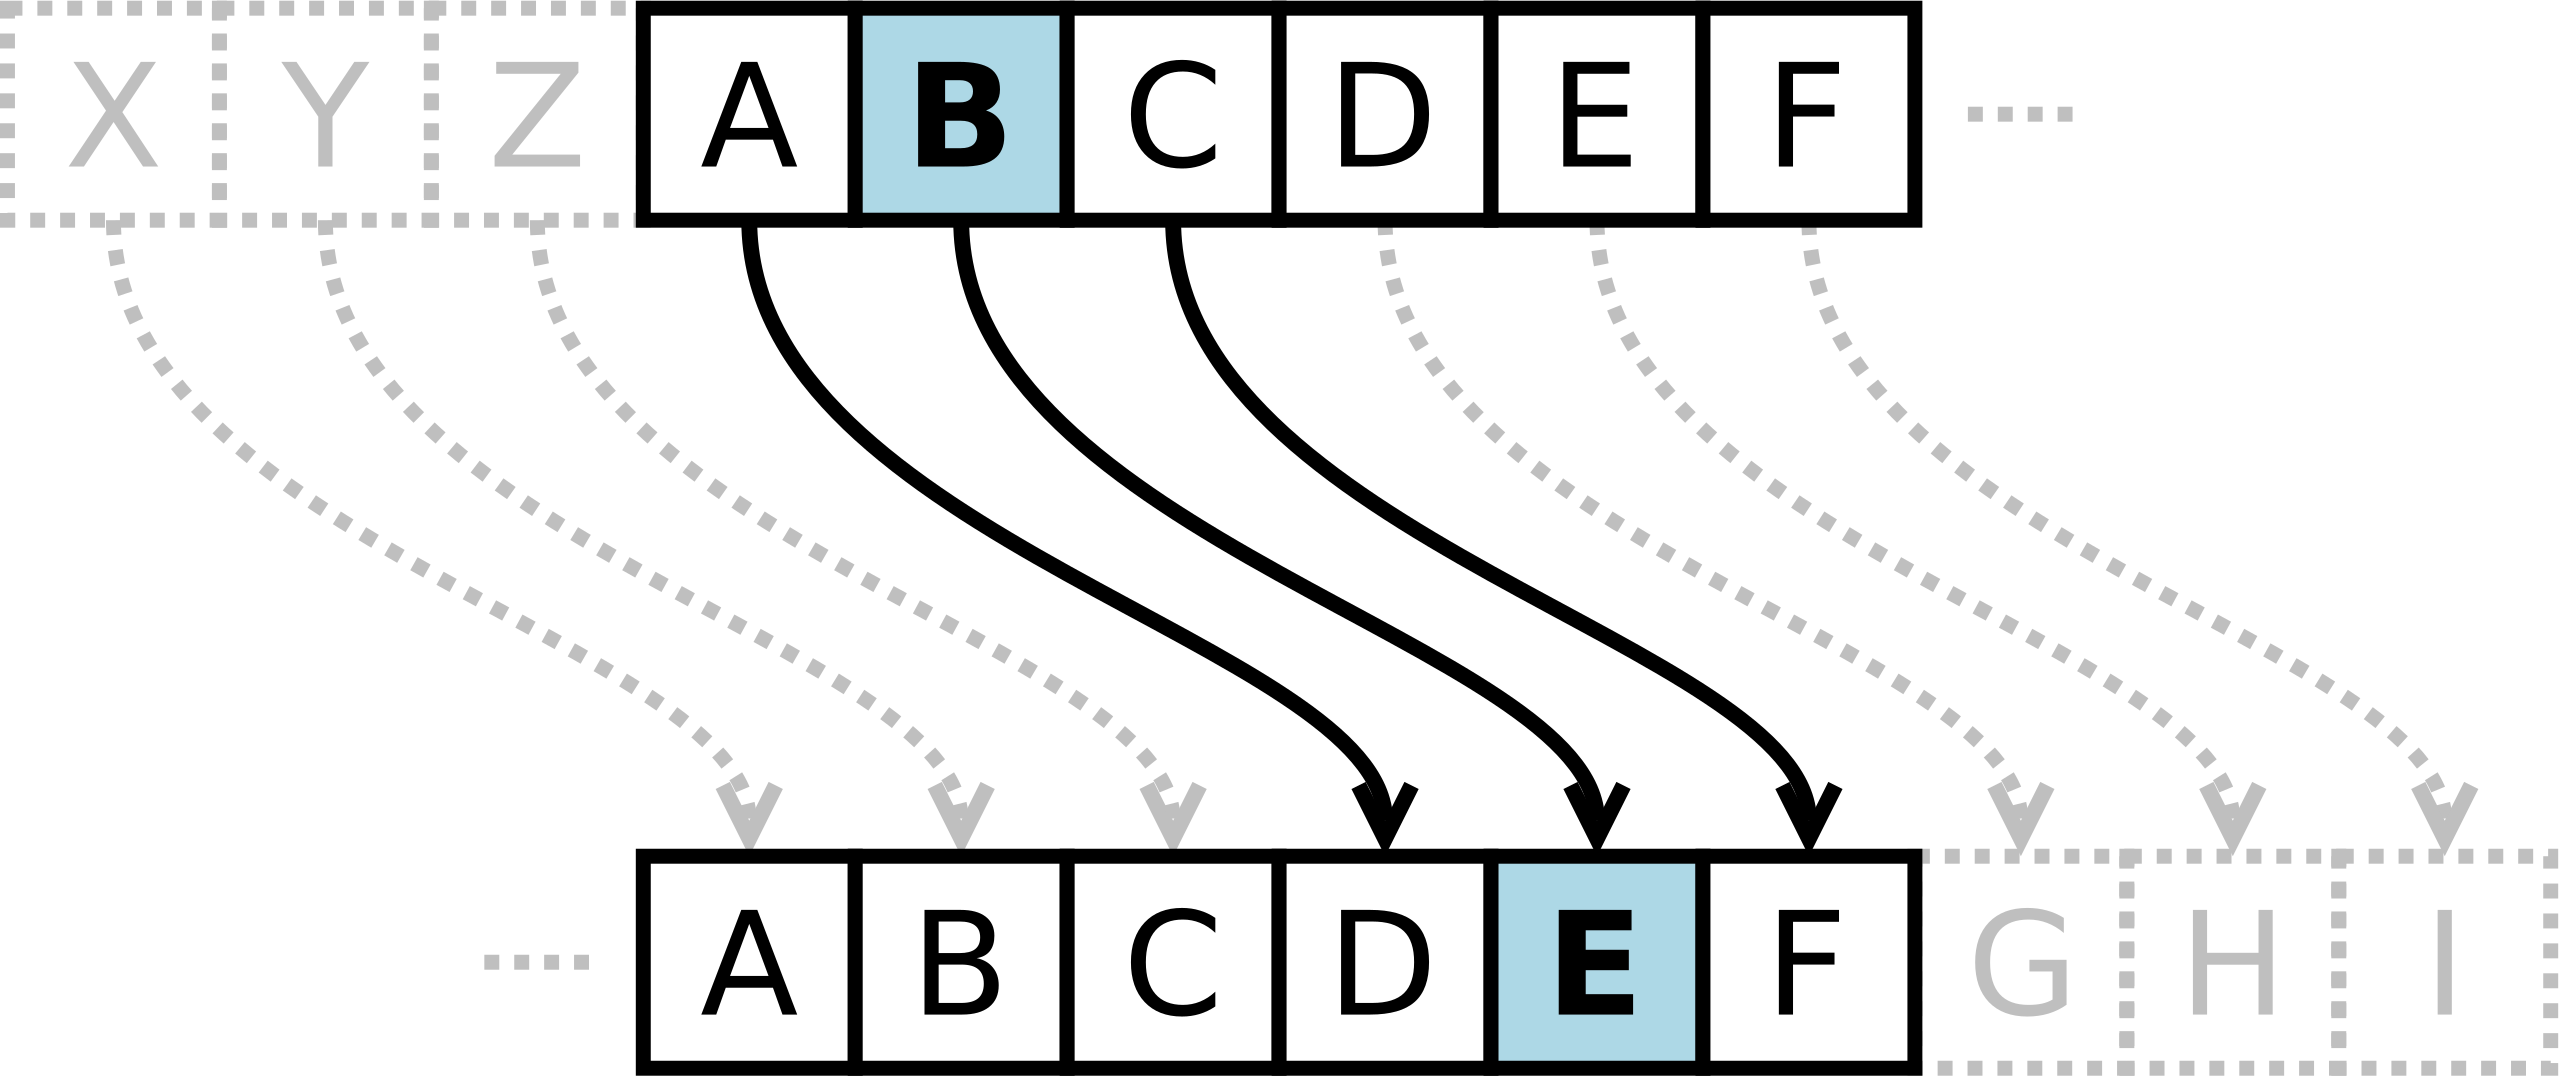
\includegraphics[width=0.4\textwidth]{caesar.png}
\end{center}
Напишите функцию \texttt{void encrypt(char* str, int k)}, которая будет зашифровывать фразу шифром Цезаря.
\begin{center}
\begin{tabular}{ c | c }
 вход & выход \\ \hline
 1 ABCZ & BCDA\\
 15 ZzZzZ & OoOoO \\
 7 The Fox Jumps Over The Dog & Aol Mve Qbtwz Vcly Aol Kvn \\
 13  Green Terra & Terra Green
\end{tabular}
\end{center}

Считывание слово за словом:
\begin{lstlisting}
int main() {
    char s[100];
    while (1) {
        scanf("%s", s);
        printf("<%s>\n", s);
    }
}
\end{lstlisting}

\item \textbf{Переворот слов:} Используйте решение задачи Переворот, чтобы перевернуть каждое слово в строке.
\begin{center}
\begin{tabular}{ c | c }
 вход & выход \\ \hline
 The Fox Jumps Over The Dog & ehT xoF spmuJ revO ehT goD \\
\end{tabular}
\end{center}


\item \textbf{Умножение на 3:} На вход передаётся целое положительное число $n < 10^{10000}$. Нужно напечатать это число, умноженное на 3.
\begin{center}
\begin{tabular}{ c | c }
 вход & выход \\ \hline
  1234567890987654321234567890987654321 & 3703703672962962963703703672962962963 \\
 
\end{tabular}
\end{center}

\item \textbf{Сортировка символов:} Отсортируйте символы строки.
\begin{center}
\begin{tabular}{ c | c }
 вход & выход \\ \hline
 MIPT & IMPT \\
 Majestic12 & 12Maceijst \\
 The Fox Jumps Over The Dog & \quad \quad \quad DFJOTTeeeghhmooprsuvx \\
\end{tabular}
\end{center}

\end{itemize}

\subsection{Строки. Стандартные функции библиотеки \texttt{string.h}:}
\begin{itemize}
\item \texttt{unsigned int strlen(char* str)} - возвращает длину строки
\item \texttt{char* strcpy (char* a, char* b))} - копирует строку b в строку a, т.е. a = b.
\item \texttt{int strcmp(const char* a, char* b)} - лексикографическое сравнение строк (возвращает 0, если строки одинаковые, положительное, если первая строка больше, и отрицательное, если меньше)
\item \texttt{char* strcat(char* a, char* b)} - приклевает копию строки b к строке a.
\item \texttt{char* strstr(char* a, char* b)} - ищет строку \texttt{b} в строке \texttt{a}. Возвращает указатель на первый символ вхождения строки \texttt{b} или \texttt{0 (NULL)} если такой строки нет.
\end{itemize}
\begin{lstlisting}
#include <stdio.h>
#include <string.h>
int main() {
	char a[100] = "Dog";
	char b[100] = "Mice";
	// Строки это массивы, поэтому их нельзя просто присваивать 
	//( можно только при инициализации )
	a = "Cat"; // Это не будет работать! Нужно использовать strcpy:
	strcpy(a, "Cat");
	
	// Строки это массивы, поэтому их нельзя просто сравнивать
	a == b; // Это не будет работать! Нужно использовать strcmp:
	printf("%d\n", strcmp(a, b)); 
	// Напечатает -1 так как a < b, то есть "Cat" < "Mice", т.к. 'C' < 'M'
	
	// Конкатенация ( склейка ) строк. Можно воспринимать как +=
	strcat(a, b);
	printf("%s\n", a); // Напечатает CatMice
}
\end{lstlisting}

\begin{itemize}
\item \textbf{Обмен строк:} Напишите функцию \texttt{void swap\_strings(char* a, char* b)}, которая будет обменивать значениями две строки. Используйте стандартную функцию \texttt{strcpy}. Предполагается, что размер каждой из строк ограничен 100 символами.
\item \textbf{Поиск подстроки:} Считать 2 строки и проверить является ли вторая строка подстрокой первой строки. Вывести на экран YES или NO соответственно.
\end{itemize}
\begin{lstlisting}
#include <stdio.h>
#include <string.h>
int main() {
    // Массивы строк - это двумерные массивы чисел типа char
    char words[500][100];
}
\end{lstlisting}
\begin{itemize}
\item \textbf{Массив слов:} Напишите программу, которая будет считывать слово за словом и записывать их в массив \texttt{words}. Программа должна заканчиваться когда пользователь напишет слово \texttt{exit}. После этого все слова должны быть напечатаны на экран через пробел. 
\item \textbf{Сортировка слов:} Напишите программу, которая будет считывать слово за словом и записывать их в массив \texttt{words}. Программа должна заканчиваться когда пользователь напишет слово \texttt{exit}. После этого все слова должны быть напечатаны на экран в отсортированном виде.
\end{itemize}

\end{document}